
Kõige sobivama mudeli valimisel lähtuti inferentsi kiirusest ja mudeli täpsusest objektide hindamisel. Kõik katsed on läbi viidud Jetson AGX Xavier 32 GB masina peal. Mudelite hindamise katsed on läbi viidud ideaaltingimustes, mis välistab kõikvõimalikud faktorid, mis võivad hinnatava mudeli testimise tulemustes hälbeid tekitada.

Antud katsetes analüüsitakse ainult närvivõrgu mudeli töötlemisvõimekust, eraldatuna ülejäänud süsteemist (kaamerad ning nendelt tulevate kaadrite eeltöötlus ning kaadritele tuvastatud objektide informatsiooni kuvamine ning edastamine teistele süsteemidele), et saada kõige optimaalsem ning hälbevaba tulemus mudelite jõudluse ning riistvara utiliseerituse kohta.

\section{Katsete läbiviimine}\label{katsete-luxe4biviimine}

Katsete läbiviimise keskkond vastab järgnevatele tingimustele:

\begin{enumerate}
\def\labelenumi{\arabic{enumi}.}
\item
  Inferentsil kasutatavad kaadrid on spetsiifiliselt välja valitud, standardiseeritud ning enne testi algust ettevalmistatud ehk närvivõrgu sisendi suuruse jaoks skaleeritud ning eeltöödeldud. See välistab igasuguse lisatöö ja koormuse graafikakaardile ja protsessorile mis mõjutaks närvivõrgu tööd negatiivselt ning võimaldab kõiki katsetatavaid mudeleid hinnata samaväärselt ühise andmestiku peal.
\item
  Katsetatavad mudelid on enne testjooksu läbiviimist riistvaraliselt eelsoojenduse faasi läbinud ehk on täielikult masina graafikakaardi mällu loetud ja läbinud 50 kalibreerimise inferentsi iteratsiooni, kasutades eelnevalt mainitud ette valmistatud testkaadreid, see võimaldab mudelite testfaasi jaoks luua keskkonna kus kõik mudelid on võrdselt ette valmistatud ning valmis töötama oma maksimaalsel võimekusel.
\item
  Testjooksude arv on 1000, mille jooksul mõõdetakse ette valmistatud kaadritel tehtavat inferentsi kiirust ja tuvastustäpsust.
\item
  Tuvastustäpsust hinnatakse järgmise valemiga:
\end{enumerate}

\begin{quote}
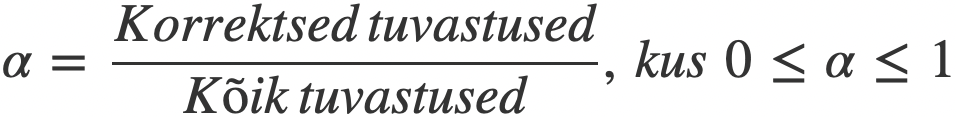
\includegraphics[width=3.18442in,height=0.37002in]{media/image23.png}

Mida lähemal tulem on ühele, seda täpsem on mudel ning suuteline tuvastama objekte.
\end{quote}

\begin{enumerate}
\def\labelenumi{\arabic{enumi}.}
\setcounter{enumi}{4}
\tightlist
\item
  Mudeli kiirust hinnatakse inferentsiks kulunud ajaga millisekundites, (graafikutel kuvatuna töödeldud kaadrite hulk ühe sekundi jooksul)
\end{enumerate}

Jetson AGX Xavieri tarkvaraline konfiguratsioon:

\begin{itemize}
\item
  JetPack 5.0.2
\item
  Ubuntu 20.04.5
\item
  kernel 5.10.104-tegra
\item
  L4T 35.1.0
\item
  Python 3.8.10
\item
  torch 1.12.0
\item
  torchvision 0.13.0
\item
  cv2 4.5.0
\item
  TensorRT 8.4.1.5
\item
  CUDA 11.4
\end{itemize}

\section{Tulemuste analüüs}\label{tulemuste-analuxfcuxfcs}

Katsed viidi läbi kahes konfiguratsioonis: ühe kaadriga ning kolme kaadriga paralleelselt protsessides, kuna toodangkeskkonnas rakendatakse kolmest kaadrist tuleva info peal närvivõrgu töötlust. Joonistel kujutatud \emph{mean Average Precision} parameeter (kollases) väljendab mudeli keskmist summaarset täpsust kõikide klasside peale kokku, see tuleneb katsetest, mis viidi läbi COCO 2017 aasta valideerimise andmestikust valitud klassidel, kus kõikidest klassidest valiti võrdne hulk testandmeid \cite{ref64}, \emph{accuracy} parameeter (punases) saavutati eraldi loodud andmestikul, mis sisaldas ainult laevu. Katsete tulemused on kujutatud mudelite suuruste ehk parameetrite hulga järgi kasvavas järjekorras, väikseim mudel vasakul, suurim paremal, et tagada intuitiivne ülevaade kõikidest parameetritest.

Suuremate sisenditega mudelite joonistel (vt Joonis 6.2.2 ja 6.2.4) tekkinud täpsuse kõikumised on põhjustatud sellest et ``6'' lõpuga mudelite skaleerimisekihid on loodud suuremate sisendresolutsioonide jaoks ning teiste mudelite kihid, väiksemate sisendresolutsioonide jaoks \cite{ref65}. Seetõttu on ka viimaste täpsus väiksem antud resolutsioonil.

Optimeeritud mudelite ja optimeerimata mudelite kiiruste vahe on vähemalt kahekordne, kõige suurem kiiruste vahe on 4,28 kordne, mudelitepaaril yolov5l6 (vt Joonis 6.2.3). Optimeeritud ning optimeerimata mudelite täpsuste vahe minimaalne (\({1,7 \cdot 10}^{- 3}\)), ehk optimeerimine täpsust oluliselt ei mõjutanud. Seetõttu graafikul algselt kuvatud täpsuste väärtused olid ülekattega, mistõttu kuvatakse nende keskmistatud väärtusi.

\begin{figure}[H]
\centering
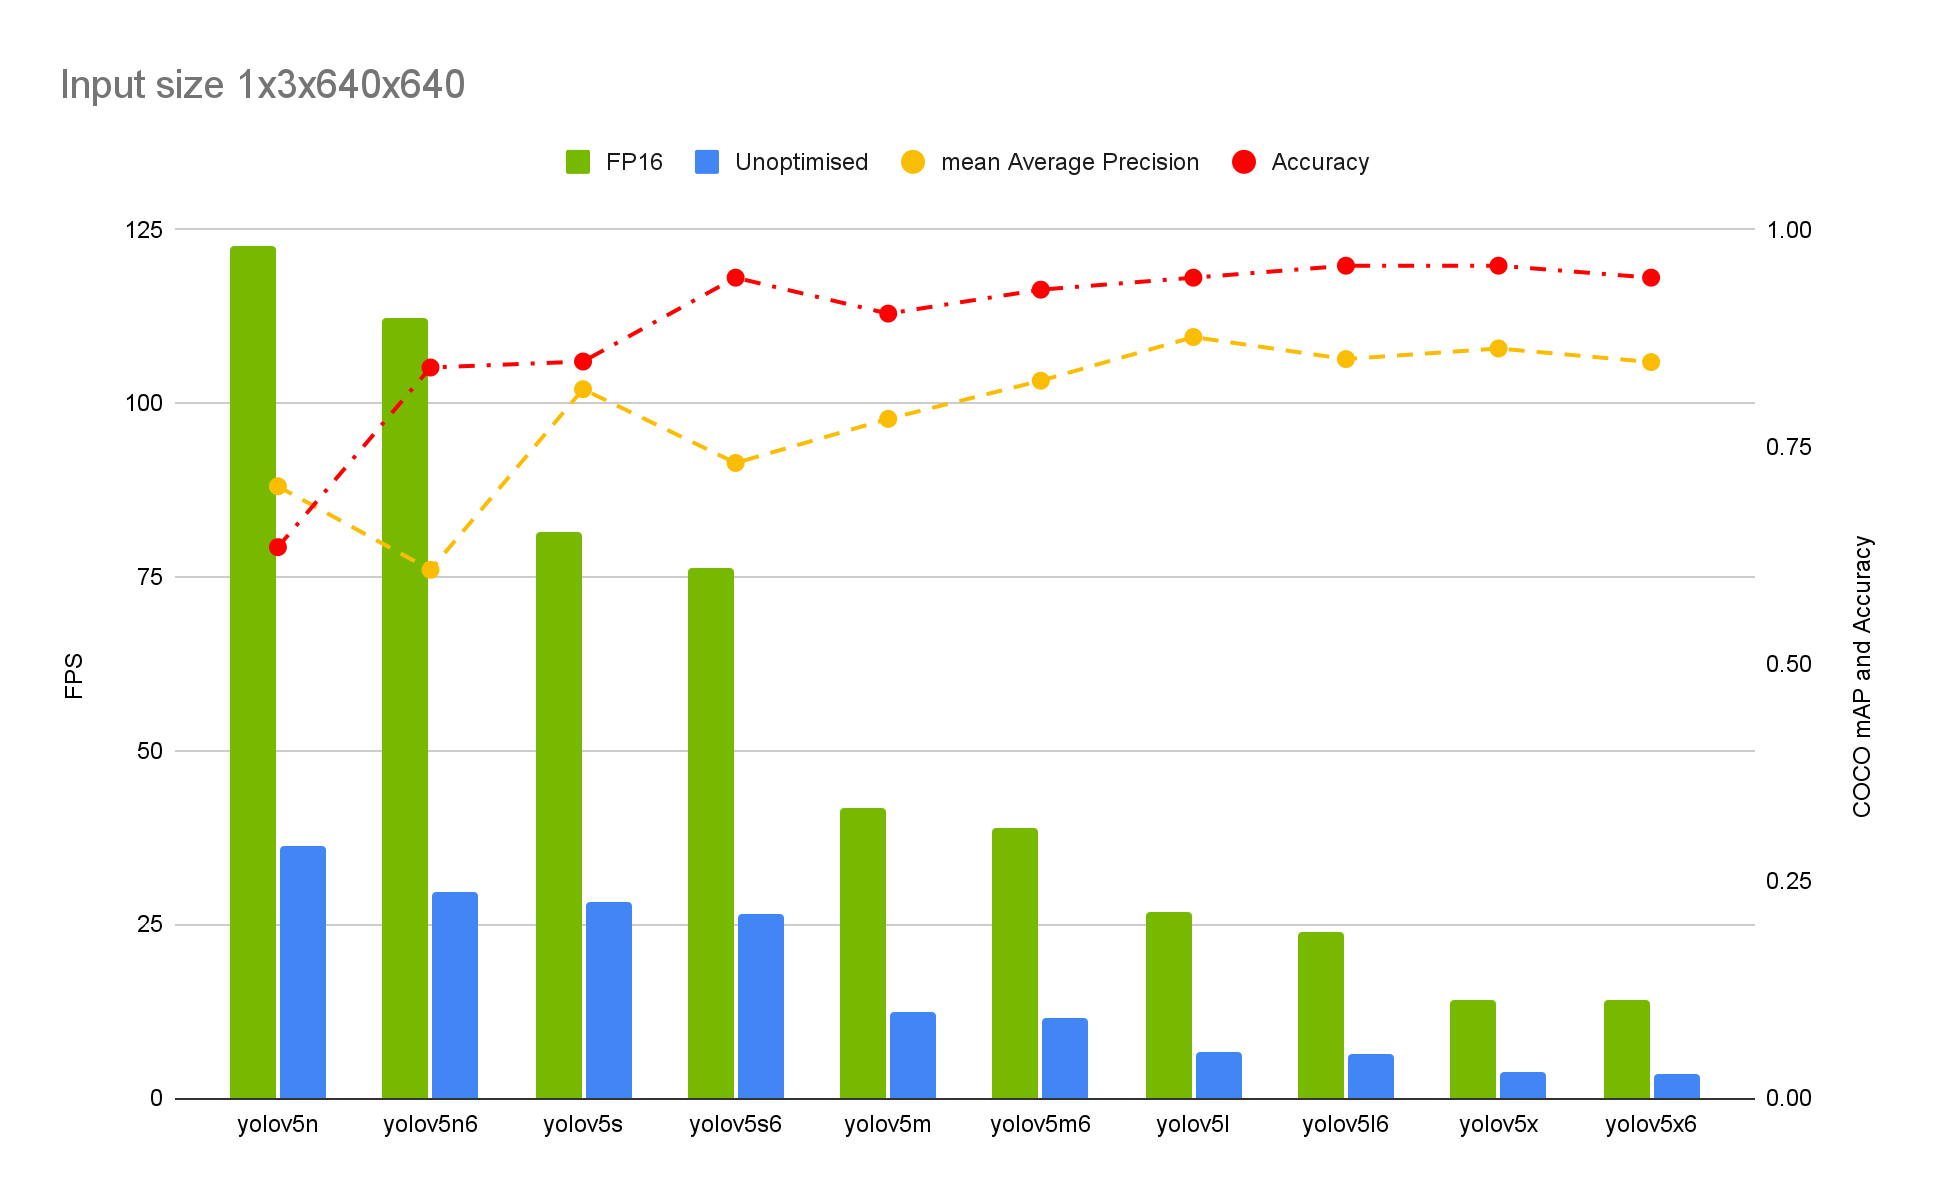
\includegraphics[width=6.10174in,height=3.77778in,alt={Input size 1x3x640x640}]{media/image24.png}
\caption{Joonis 6.2.1. Mudelite jõudlus 1 kaadri sisendiga, suurusel 640x640 pikslit}
\end{figure}

Kiireima ja aeglaseima optimeeritud mudeli kiiruste vahe on 108 kaadrit sekundis, kusjuures parim kiirendus neljakordne. Keskmine optimeeritud kiiruste vahe 3,5 kordne. Mudelite täpsus kasvab YOLOv5l mudelini ning sealt edasi olulist täpsuse kasvu ei ole, seega sellest mudelist alates kiiruse ja täpsuse suhe väheneb.

\begin{figure}[H]
\centering
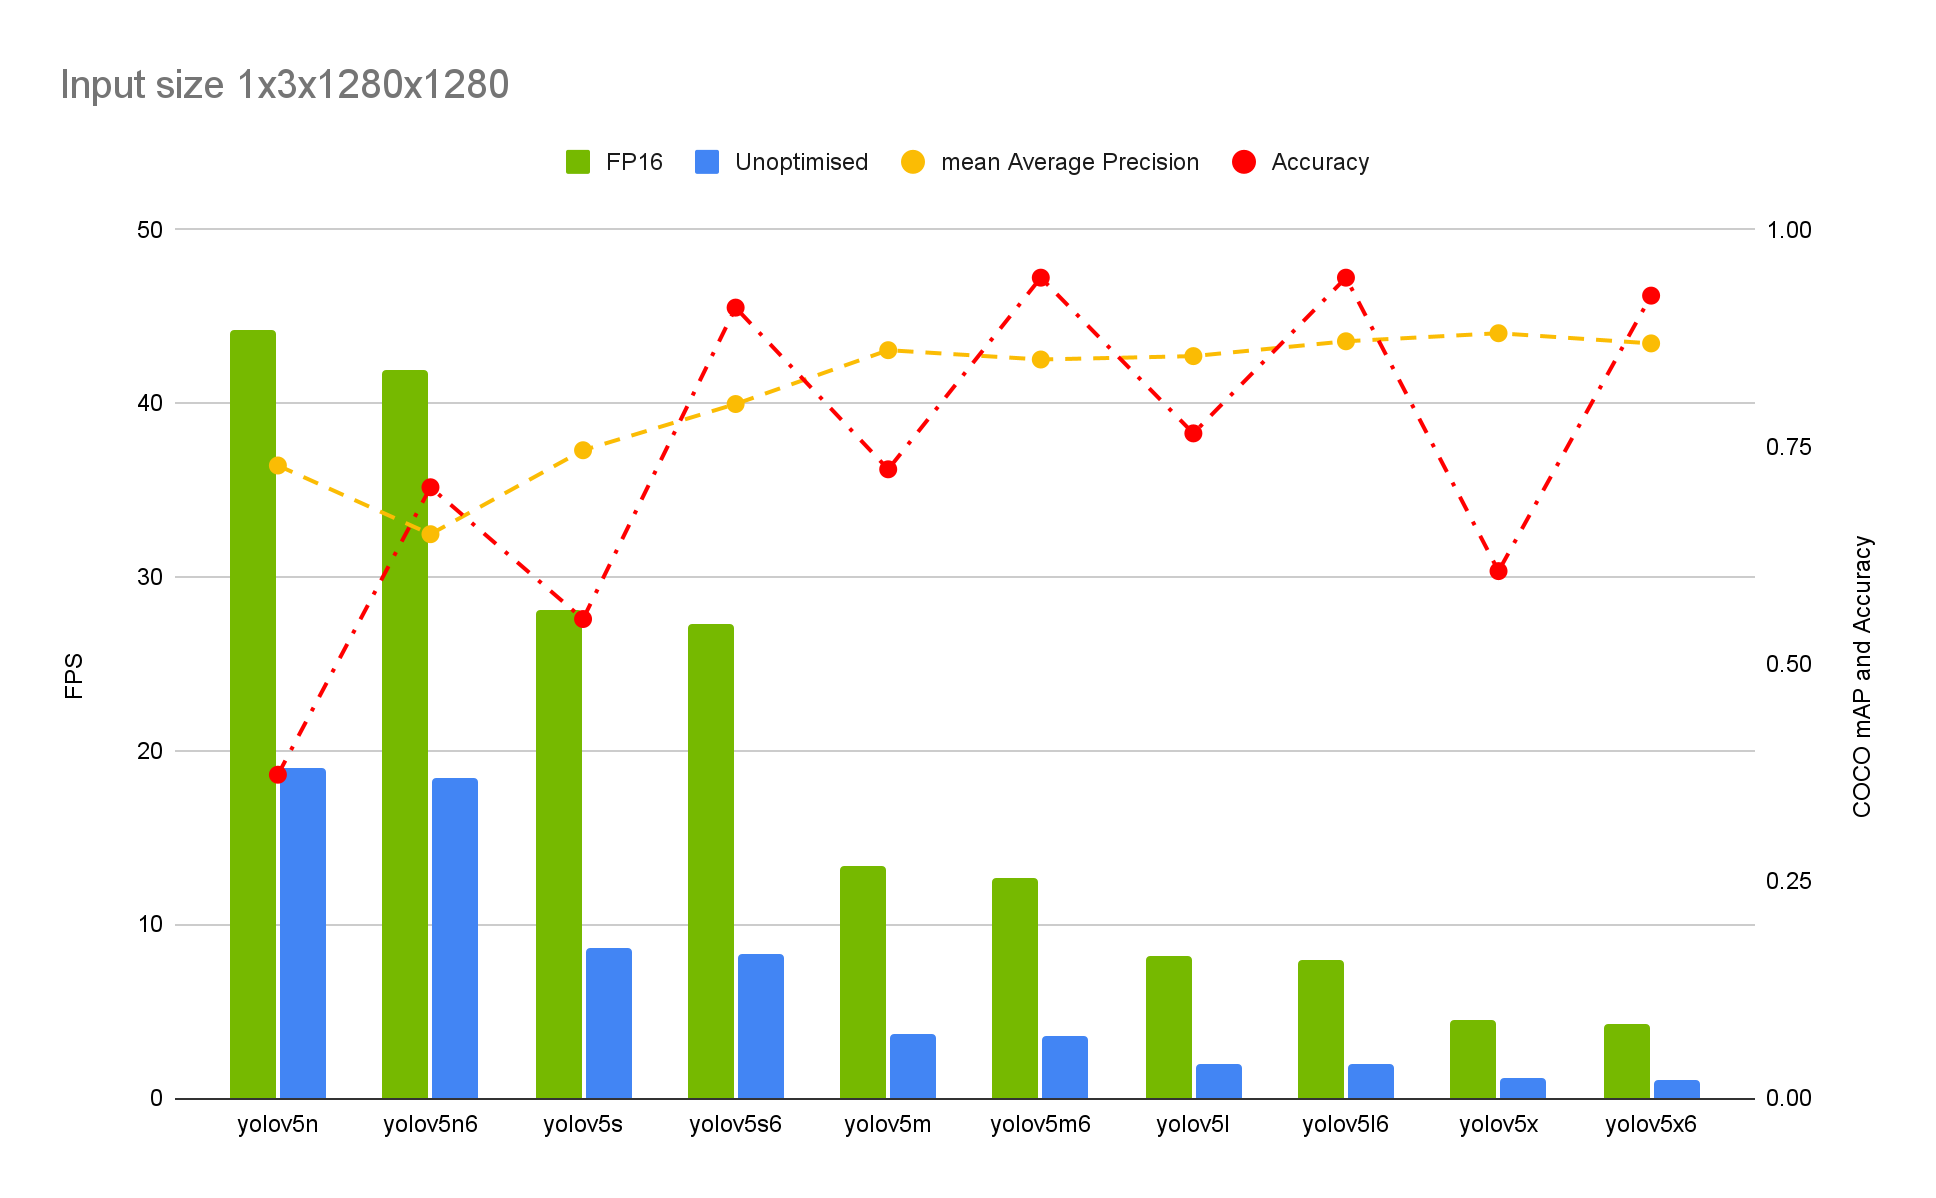
\includegraphics[width=6.10174in,height=3.77778in,alt={Input size 1x3x1280x1280}]{media/image25.png}
\caption{Joonis 6.2.2. Mudelite jõudlus 1 kaadri sisendiga, suurusel 1280x1280 pikslit}
\end{figure}

Kiireima ja aeglaseima optimeeritud mudeli kiiruste vahe on 40 kaadrit sekundis, parim kiirendus 4,1 kordne. Keskmine optimeeritud kiiruste vahe 3,5 kordne. Mudelite täpsus kasvab YOLOv5m mudelini ning sealt edasi olulist täpsuse kasvu ei ole, seega sellest mudelist alates kiiruse ja täpsuse suhe väheneb.

Ühe sisendiga 640x640 ja 1280x1280 resolutsiooniga mudelite kiiruste keskmine vahe on 36 kaadrit sekundis.

\begin{figure}[H]
\centering
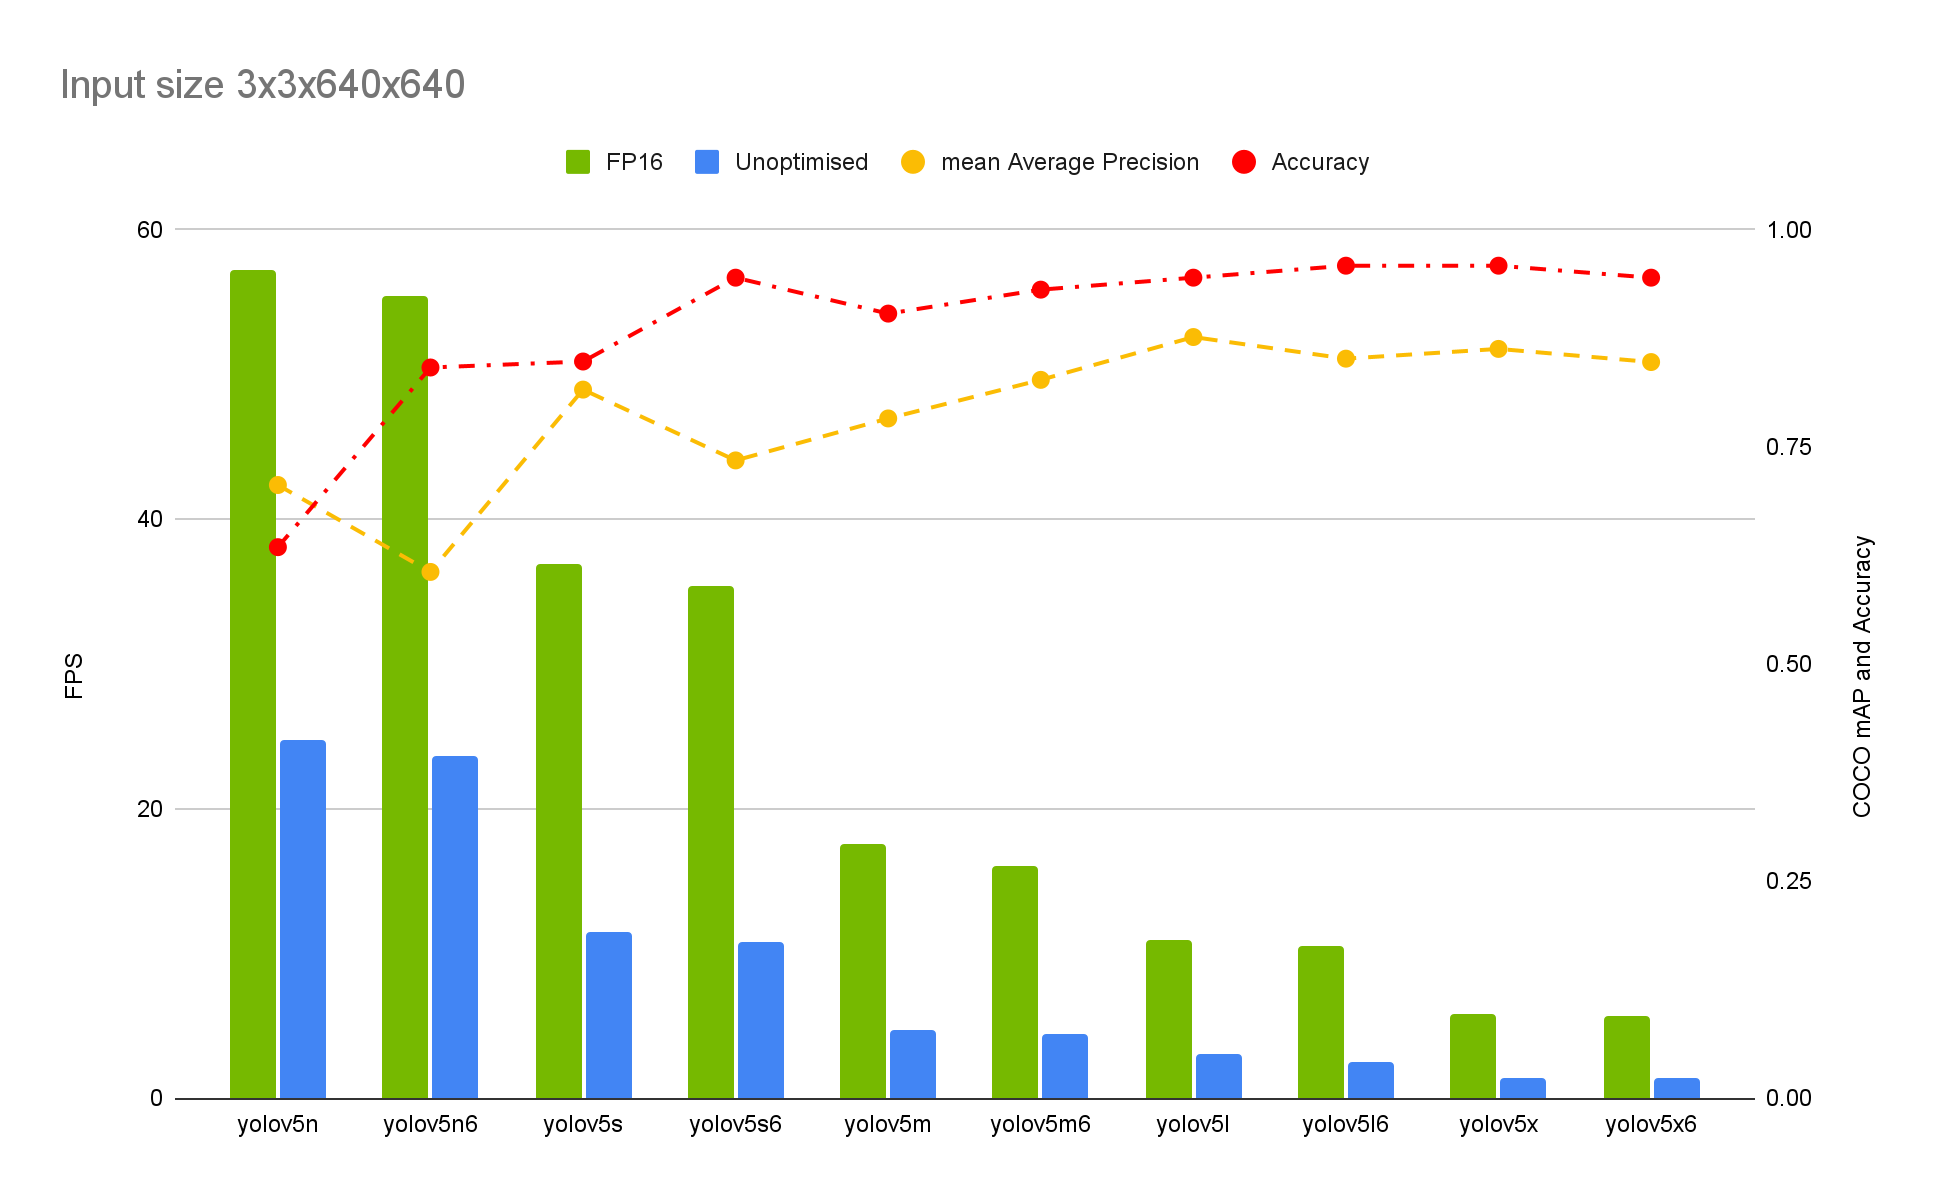
\includegraphics[width=6.10174in,height=3.77778in,alt={Input size 3x3x640x640}]{media/image26.png}
\caption{Joonis 6.2.3. Mudelite jõudlus 3 kaadri sisendiga paralleelselt, suurusel 640x640 pikslit}
\end{figure}

Kiireima ja aeglaseima optimeeritud mudeli kiiruste vahe on 52 kaadrit sekundis, parim kiirendus 4,3 kordne. Keskmine optimeeritud kiiruste vahe 3,4 kordne. Mudelite täpsus kasvab YOLOv5l mudelini ning sealt edasi olulist täpsuse kasvu ei ole, seega sellest mudelist alates kiiruse ja täpsuse suhe väheneb.

Kolme sisendiga resolutsiooniga 640x640 mudelid on keskmiselt 1,4 korda kiiremad kui ühe sisendiga sama resolutsiooniga mudelid.

\begin{figure}
\centering
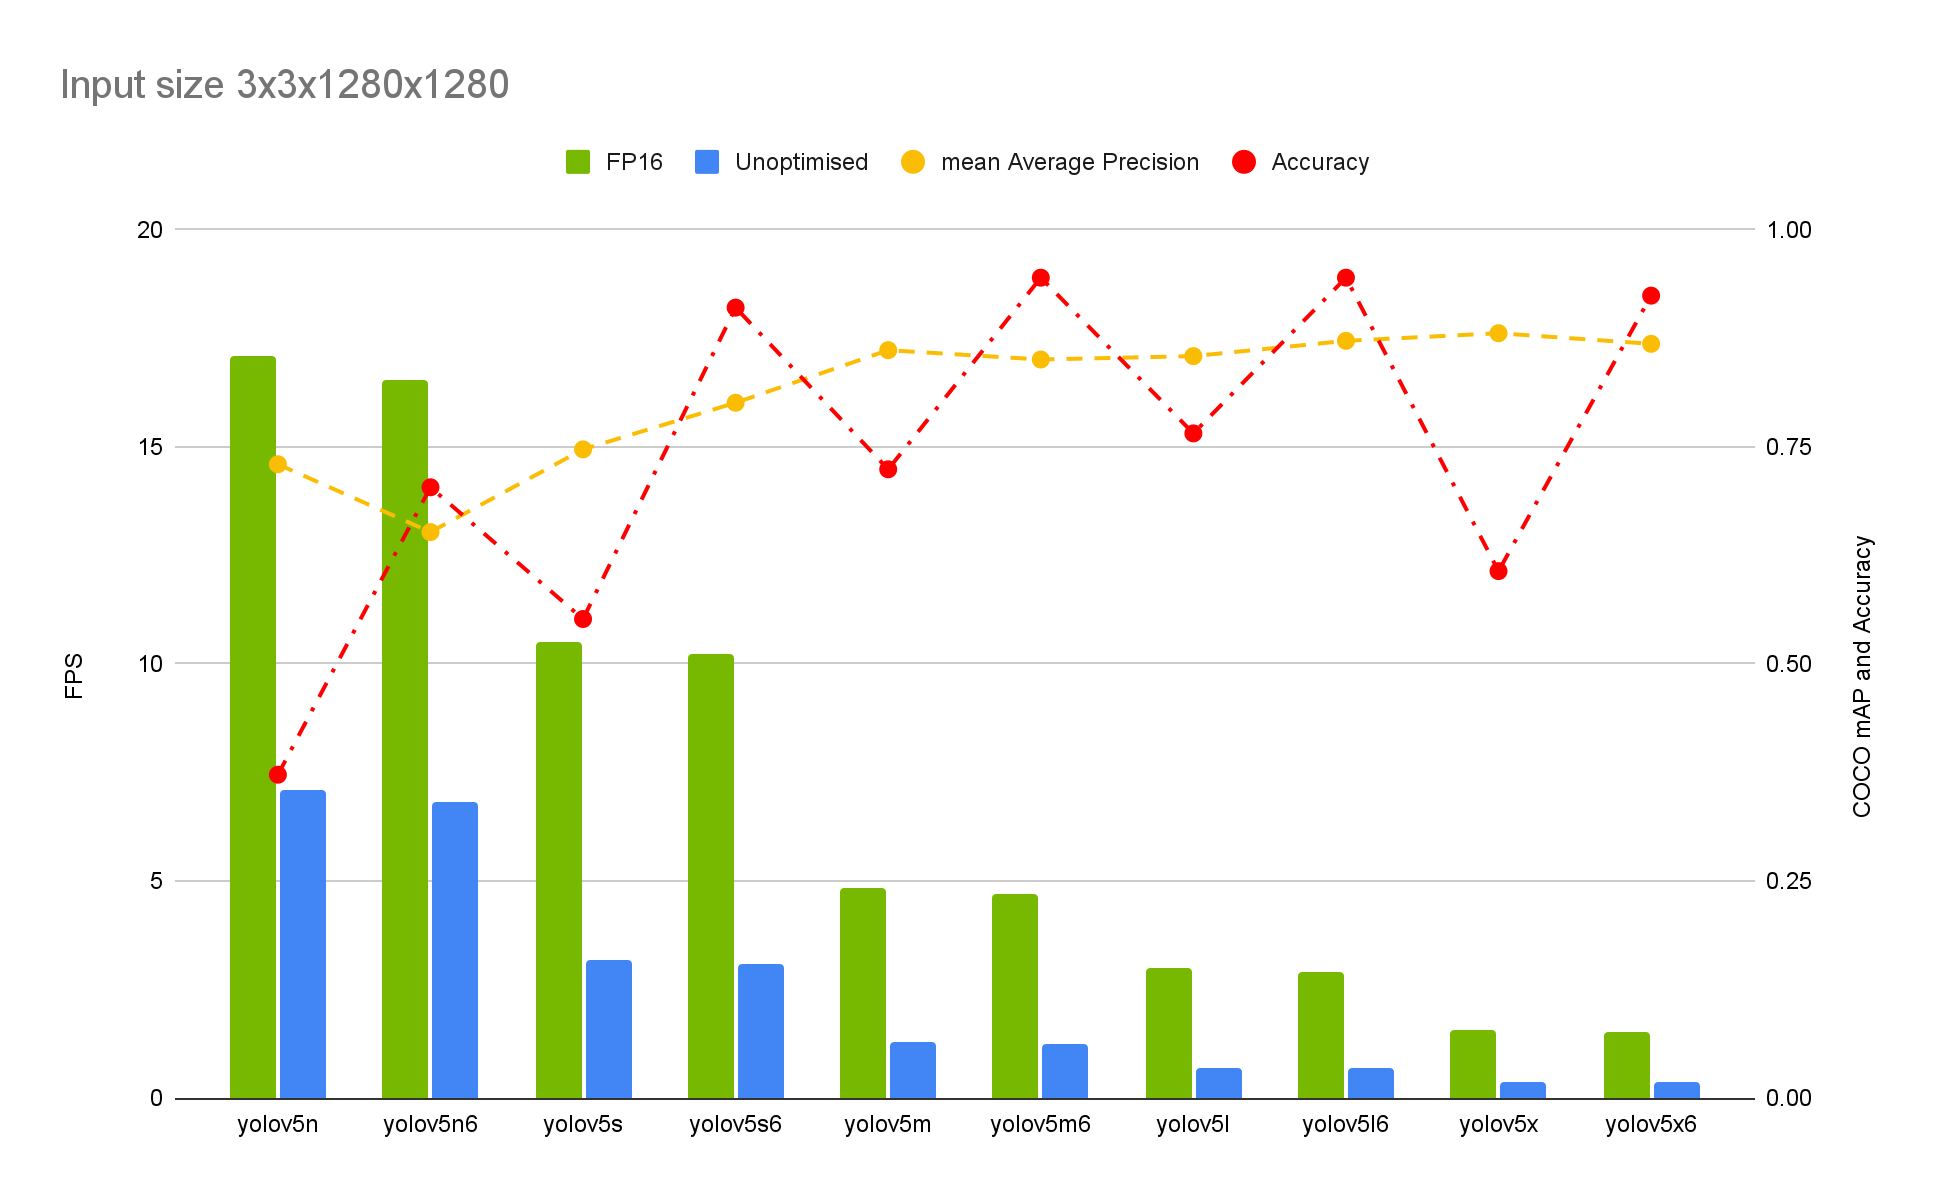
\includegraphics[width=6.10174in,height=3.77778in,alt={Input size 3x3x1280x1280}]{media/image27.png}
\caption{Joonis 6.2.4. Mudelite jõudlus 3 kaadri sisendiga paralleelselt, suurusel 1280x1280 pikslit}
\end{figure}

Kiireima ja aeglaseima optimeeritud mudeli kiiruste vahe 16 kaadrit sekundis, parim kiirendus 4,2 kordne. Keskmine optimeeritud mudelite kiiruste vahe 3,5 kordne. Mudelite täpsus kasvab YOLOv5m mudelini ning sealt edasi olulist täpsuse kasvu ei ole, seega sellest mudelist alates kiiruse ja täpsuse suhe väheneb. Antud juhul on tegemist 1,1 korda kiiremate mudelitega, võrreldes ühe sisendiga mudeleid, samal resolutsioonil.

Kolme sisendiga 640x640 ja 1280x1280 resolutsiooniga mudelite kiiruste keskmine vahe on 18 kaadrit sekundis.

Kolme sisendiga mudelid on keskmiselt 1,2 korda kiiremad kui ühe sisendiga mudelid.
